\documentclass[10pt,a4paper]{book}
\usepackage[utf8]{inputenc}
\usepackage[french]{babel}
\usepackage[T1]{fontenc}
\usepackage{amsmath}
\usepackage{amsfonts}
\usepackage{amssymb}
\usepackage{graphicx}
\author{ Antoine Robin}
\title{Warhammer - campagne}
\newcommand{\nomadversaire}{Loge des yeux écarlates}
\begin{document}
\maketitle
\tableofcontents
\chapter{Arcs narratifs}
\section{Arc principal : l'influence du chaos}
Au cours de cette campagne, les PJs vont affronter l'influence pernicieuse, mais subtile d'un culte du chaos, jusqu'au déclenchement de ses plans machiavéliques.
\subsection{Synopsis}
 C'est un arc narratif en trois actes : lors du premier, les actes du culte seront très subtils, plus une menace de fond. Lors du second, les personnages auront été mis au courant de l'existence du culte, et pourront plus précisément enquêter à ce sujet. Enfin, lors du troisième, le culte se sentant menacé, va déclencher un plan plus important pour semer le chaos.
\subsection{\nomadversaire}
 Il s'agit d'un culte lié au dieu du sang, aux rituels sanglants, mais particulièrement discrets. En effet, ses membres, d'un niveau social parfois assez haut, réalisent leurs rituels hors des villes et villages, dans les bois ou les réserves de chasses.
 
 Leurs croyances sont liées à la nature primale de la chasse, avec un tour très sombre : leurs proies sont souvent humaines, et son dévorées par la suite. Comme beaucoup de cultes de Khorne, bon nombre de leurs adeptes sont des tueurs très efficace. 
 
 La cellule de Waldenheim est dirigée par le Ritter Friedrich Reger, un noble de rang moyen, mais qui dispose d'une très bonné réputation de combattant, ayant été récemment blessé non loin de Middenheim lors du siège de la ville. Quand il n'est pas sur son domaine, à deux jours de Waldenheim, il en profite pour coordonner certaines activités. En particulier ces derniers temps, l'arrivée des PJs et leurs actions contre les forces du chaos le préoccupent, et il compte si possible s'en débarasser au plus vite.
\subsection{Acte 1 : une présence discrète}
Cet acte sera assez flou, peu de vrai structure. En effet, il s'agit de plans et d'actions du culte que les personnages pourraient rencontrer, mais sans forcément voir le point commun.

La première rencontre des personnages avec le culte, même s'ils n'en auront pas conscience immédiatement, est le bailli, qui assiste les forces du chaos dans la région en leur donnant des informations, et obéi à ses maîtres de la secte. En particulier, il a guidé les récentes attaques, et a reçu l'ordre de faire sacrifier quelqu'un d'important aux dieux noirs, afin d'apporter la faveur des dieux sombres sur les envahisseurs. Après une embuscade échouée à cause des PJs(session 3), il a donc fait enlever la Ritterin von Hauptberg, et l'a livrée aux créatures de la forêt, qui s'apprêtent à la sacrifier. Il s'agira d'un combat livré à la lueur des torches, près d'une pierre de sacrifice, apparemment certains plutôt récents. Une fois ce péril vaincu, les personnages gagneront ??? PX.

La seconde rencontre aura lieu au bal : le ritter a engagés une paire de mutants particulièrement dangereux, qui servent de gros bras au culte. Lui-même et un serviteur de confiance doivent leurs permettre d'embusquer les PJs, pour tenter de s'en débarrasser.
\subsection{Acte 2 : un culte mystérieux}
Cet acte commence quand les personnages sont mis au courant de l'existence de ce culte, et peuvent commencer à relier les points entre certains problèmes de l'acte 1. Cela va permettre aux PJs d'enquêter beaucoup plus spécifiquement, d'après les indices qu'ils ont pu obtenir, et qu'on a pu leur donner le cas échéant.
\subsection{Acte 3 : le plan machiavélique}
Suite à l'enquête des PJs, et leur lutte contre \nomadversaire, ce culte se sent menacé, et commence à réagir beaucoup plus violemment : il ordonne la mort des PJs et commence à déclencher son plan global. Cela va amener les PJs à voyager dans l'empire pour lutter contre le coeur du culte.
\section{Arcs secondaires}
\subsection{Les marais de Schadensumpf}
Ces marais, difficiles d'accès, sont remplis de créatures et de problèmes, et les PJs pourraient avoir plusieurs raisons de s'y diriger : explorer des pistes pour enquête, chercher une ancienne relique perdue.... Au nord de ces marais, les collines embrumées, qui peuvent également receler des intérêts.
\subsection{Familles criminelles}
Trois groupes criminels sont rivaux dans la ville de Waldenheim et ses environs immédiats. L'un gère essentiellement les docks, l'autre ce qui se passe dans les faubourgs de la ville, au sud des remparts, et enfin, le troisième défend son territoire près du marché à l'ouest de la ville. En plus de leur rivalité latente, il peut y avoir des problèmes plus importants

Orloff : faubourgs

Stahlers : quais; basé  au \emph{repos fluvial}, une taverne des quais où ils gèrent des paris plus ou moins clandestins. Ils organisent cela dans une arrière-salle, plus animée que la salle principale. Le contact de Johannes est un certain Otto (?)
\subsection{Sous Waldenheim}
La forteresse du clan Volkn, des skavens, se trouve sous la région, et des groupes d'éclaireurs et de pillards peuvent rôder dans le coin. En particulier, les PJs pourraient se retrouver face à ces différents groupes, ou se mettre en travers du chemin du chef de guerre du clan, Skarrik tranche-pattes.
\subsection{Les familles von Hauptberg et Oberstein}

Deux familles importantes de Waldenheim, qui sont régulièrement en conflit sur de nombreux sujets. Aujourd'hui les Oberstein ont le titre de comtes de Waldenheim, et les von Hauptberg font parti de la noblesse importante de la région, et sont une épine permanente dans leur flanc.

Les personnages pourraient sans doute être recrutés dans la maisonnée de l'une ou l'autre de ces familles, ce qui pourrait fournir de nombreuses occasions de découvrir les lieux et de travailler.

Une option est de faire rencontrer un membre d'une des maisons dans la première mission, qui pourrait leur proposer un travail.

Plus tard, le conflit entre les deux familles peut s'envenimer : duels de justice (truqués), affrontements plus ou moins violents, et une tentative d'assassinat (perpétrée par une autre faction ?). Bref, les personnages ne devraient pas trop manquer de travail à accomplir pour leur patron.

L'espionnage est une possibilité, avec la corruption d'un PJ pour obtenir des informations par un autre de leurs contacts.

Les von haupberg portent une livrée verte et noire.

\subsection{Le rassemblement de la horde}
Vaguement soutenu par les forces du culte, et profitant des trainards de la horde d'archaon, Morghast le désosseur commence à se tailler un nom dans la région : il commence à rassembler des créatures de tout type et de toute forme dans la Drakwald, sous sa bannière corrompue.

Celles-ci vont menacer les villages de la région, notamment Utingen, et formeront un adversaire adequat pour le début de campagne, avant que les PJs ne tuent leur seigneur dans un affrontement violent. 

Un arc en plusieurs parties : une partie sous la menace de la horde, une course avec celle-ci pour un lieu ou artefact, et enfin, une recherche du seigneur de la horde pour le tuer.

\subsection{Le bal des von Hauptberg}
Le bal va se dérouler au manoir des von Haupberg, et a pour but de présenter à toute la bonne société de la ville le nouveau membre des von hauptberg, en tant que 'cousin' du freiherr. 

Au milieu de celui-ci, le culte, via un agent pertinent, va tenter de semer le chaos, en tout cas de viser les PJs. Ceux du groupe qui ne participent pas activement à la fête auront plus de chances de surveiller cela.

\subsubsection{Invités majeurs et leurs actions}
\paragraph{Le vizgraf Oberstein} Invité de plus haut rang, il arrive sur le coup des 20h, discutera rapidement avec tout le monde en profitant de la nourriture, avant de passer une bonne partie de la soirée à discuter dans le bureau du freiherr von hauptberg.
\paragraph{La Ritterin von Hauptberg}Hôtesse de ce bal, elle s'assure que tout se passe bien : elle surveille les serviteurs, et s'assure que tout se passe au mieux pour les invités. Elle passe n peu partout pour discuter avec chacun.
\paragraph{Le freiherr von Hauptberg} Hôte de la soirée, il va essentiellement discuter avec les invités et les accueillir. La fin de la soirée sera passée dans son bureau avec le vizgraf.
\paragraph{Le capitaine Oberstein}Neveu du comte, et récemment héros militaire. Il n'apprécie pas forcément d'être chez les von Hauptberg, et va essayer d'éviter les sujets de contentieux. Il compte par contre en profiter pour discuter avec Isolde et Hartman Gehlen, au sujet de ses fiançailles. Il sera là à partir de 19h30.
\paragraph{Barundin Obarad} Représentant des clans nains de Karak Izor, il sera là toute la soirée à partir de 20h. Il souhaite rencontrer le nouveau membre des von Hauptberg, et peut-être rencontrer le tueur nain qui a fait parler de lui en ville. Il peut aussi chercher de l'assistance pour discuter avec le vizgraf.
\paragraph{Oskar Ulfenwacht}Représentant du clergé d'Ulric à . Il arrive tôt, vers 18h, et sera parti tôt(21h). C'est un homme direct, qui souhaite en savoir plus sur les PJs. Il se montre en particulier curieux quand à Aldemar, vis-à-vis des archives de sa famille.
\paragraph{Leopold Müller}mage des cieux de Waldenheim, présent pour discuter quelque peu avec le vizgraf, il sera là entre 18h et 20h30. Il est curieux d'en apprendre plus sur les hommes-bêtes, mais craint que ceux-ci ne soient pas les menaces qu'il a entraperçu dans les étoiles.
\paragraph{Ritter Friedrich Reger} Héros de guerre, récemment revenu des combats de Middenheim. Il a fait entrer deux mutants particulièrement dangereux pour tuer les PJs lors de la fête.
\paragraph{Isolde et Hartman Gehlen} Hartman est représentant de la puissante guilde des tisserands, teinturiers et tailleurs de Waldenheim, et souhaite se montrer sous son meilleur jour. Sa fille, Isolde, est fiancée au capitaine Oberstein, leur mariage étant prévu à la fin de l'été. Ils seront là toute la soirée, à partir de 19h.
\paragraph{Elma Buchmacher}Elma représente fréquemment sa guilde, celle des marchands, auprès de la noblesse de la ville. Elle dispose de bonnes informations, et de contacts dans tout le middenland, ainsi qu'à Marienburg. Elle possède la librairie Chez Elma sur la KurzStrasse.
\paragraph{Konrad Frenz} Un petit nobles des environs de la ville, c'est surtout un paumé, reconnu comme tel par la majeure partie de la ville. Si il n'est pas surveillé, il finira sans doute par s'effondrer, trop alcoolisé, dans un coin, mais peut causer un esclandre avant cela.
\subsubsection{Déroulement prévu}
\paragraph{18h} ouverture du bal, et arrivée des premiers invités. Leopold Müller et Oskar Ulfenwacht font partie de ceux-ci. Oskar ira discuter avec les PJs directement.
\paragraph{19h} la majeure partie des invités arrivent, essentiellement de la petite noblesse ou haute bourgeoisie de la ville. Elma Buchmacher, Konrad, le ritter Reger et les Gehlen en font partie. Leopold essaie d'avoir plus d'informations des PJs sur ce qu'ils ont affrontés, il s'agit d'un léger impair de protocole, mais c'est un mage. Reger ira aussi en apprendre un peu plus, jouant sur son propre statut de vétéran.
\paragraph{20h}quelques invités arrivent encore, notamment le vizgraf et Obarad. Oskar et Elma discutent dans les jardins. Friedrich et Leopold, en froid, se croisent, avant que Leopold ne quitte la soirée. 
\paragraph{20h30}Konrad et Obarad peuvent créer un esclandre, le premier se ridiculisant d'abord par sa maladresse, puis par son impolitesse. Profitant de cela, Friedrich fait rentrer ses deux mutants par une porte dérobée.
\paragraph{21h} Un serviteur vient demander les PJs, apparemment un invité cause des troubles dans les jardins. Il s'agit d'une tentative d'embuscade par les deux mutants.
\subsubsection{Rumeurs du bal, et où les obtenir}
\paragraph{En discutant avec les invités}Apparemment, la famille de Konrad souhaiterai le faire engager dans l'armée (vrai). Cela fait longtemps que la Ritterin n'avait pas passé plus de quelques jours à Waldenheim (vrai). Les marchands de la ville vont bientôt rentrer en conflit avec les tisserands (faux). Oskar passe beaucoup de temps hors de la ville (vrai, il a eu quelques indices sur une relique perdue dans les archives des von schluschenbar). Les Gehlen n'ont pas encore commencé l'organisation du mariage d'Isolde (faux, ils sont très discrets à ce sujet).
\paragraph{En écoutant dans les jardins}La ritterin discute avec Berthold, s'inquiétant de l'état de ses blessures récentes. Oskar et Elma discutent des archives, d'un 'indice', et du fait que la majeure partie doit toujours être cachée. Isolde et le capitaine sont ensemble, apparemment amoureux. Friedrich déverrouille une porte menant vers l'extérieur, et s'éclipse quelques instants. Barundin discute avec Leopold des dangers qui peuvent peser sur la ville.
\paragraph{Bruits de couloirs}Le vizgraf et le frieherr discutent devant une partie de Trônes (un jeu de carte), dans le bureau du freiherr, tout en buvant de l'alcool venu d'une réserve personnelle. Hartman Gehlen essaie de discuter avec la Ritterin, qui le repousse dès que le protocol le permet.
\subsubsection{Les cultistes, et leur attaque}
Un serviteur vient, vers 21h, demander les PJs, apparemment, deux invités inquiètent les serviteurs dans les jardins. Quand les PJs arrivent, ils sont effectivement attaqués par deux mutants particulièrement dangereux. Cela peut mettre fin à la soirée, ou pas du tout, suivant la façon dont les PJs le gère.

Dans tous les cas, les PJs trouveront un symbole grossier semblable au précédent, et pourront enquêter sur ces deux mutants.

Le premier a une peau épaisse, presque comme du cuir(2 armure, -10 Ag), et a ses mains transformées en sorte de hachoirs de bouchers. La seconde cache un troisième bras (seconde attaque) et peut hurler un cri perçant (distracting). Elle est équipé d'un couteau de chasse et d'un crochet à viande.
\section{Arcs personnels}
\subsection{Linlorryn de Laurelorn :La chasse}
un bestigor est responsable de plusieurs problèmes pour l'elfe du groupe, et les PJs pourront entendre parler de lui, voir le traquer dans la drakwald.
Il porte un symbole de crâne écarlate, et dispose d'une stature peu commune.

Ambitions :
\begin{description}
\item[Court terme :]traquer et tuer l'homme-bête responsable de ses problèmes
\item[Long terme :]Eliminer les hommes-bêtes de la Drakwald (attention !)
\end{description}
\subsection{Aldemar von Schluchenbar : L'ancienne famille}
le famille du cavalier est de petite noblesse, qui a perdu au fil du temps ses possessions et titres, ce qui l'a mené lui à monter les rangs 'à la main' plutôt que pouvoir devenir officier. Il serait peut-être possible de redorer le blason de la famille, notamment en retrouvant leurs archives, dispersées après la vente de leur domaine.

Ambitions :
\begin{description}
\item[Court terme :]faire écrire une chanson sur ses exploits
\item[Long terme :]obtenir une reconnaissance impériale
\end{description}
\subsection{Unduk Umberbuckelesson Unboki La mort glorieuse}
le tueur cherche à mourir, ce qui devrait être possible : penser à inclure une galerie de créatures de plus en plus grosses à tuer, permettant de trouver une fin glorieuse. Hommes-bêtes, trolls, guerriers du chaos, minotaure, démons .....

Ambitions :
\begin{description}
\item[Court terme :]Pacifier un adversire plus grand que lui
\item[Long terme :]mourir
\end{description}
\subsection{Nelis van Egelen :Connaissances interdites}
l'érudit du groupe est suivi par les chasseurs de sorciers, qui le suspectent d'avoir certaines connaissances interdites. Il les a fuit pour éviter leur sinistre réputation. Il est peut-être possible de travailler avec eux ou de les convaincre de la bonne foi du personnage. Dans ce cas, ils pourraient devenir des alliés, ou sinon, se révéler être des problèmes récurrents.

Ambitions :
\begin{description}
\item[Court terme :]atteindre Altdorf. A voir, peut-être inclure un groupe de mages à Waldenheim, qui pourraient être convaincus.
\item[Long terme :]découvrir les origines des vents de magie (interdit ! :p)
\end{description}
\subsection{Johannes Kleinman : des relations compliquées}
bâtard de la famille von Hauptberg, en rivalité avec les comtes de Waldenheim.

A reçu la consigne de laisser passer des voyageurs ayant un écusson représentant une main squelettique (un des groupes criminels de Waldenheim).

Ambitions :
\begin{description}
\item[Court terme :]???
\item[Long terme :]???
\end{description}
\section{Arcs tertiaires}
\subsection{Une menace sur le village}
Cet arc va ouvrir la campagne, en proposant une enquête/traque.

Le Bailli du village voit les personnages arriver, et souhaite leur proposer un travail : depuis quelques temps, les bois grouillent de créatures dangereuses, et il souhaiterai, si possible, que les aventuriers aillent vérifier ce dont il s'agit. En particulier, le meunier a affirmé que des créatures rôdent près de chez lui.

En effet, des hommes-bêtes cherchent des victimes à tuer dans la région, et le moulin, un des bâtiments les plus visibles de la région, attire facilement leur convoitise.

Cela peut se traduire par une première attaque par des ungors, qui voyaient cela comme une cible facile. Leurs traces peuvent ensuite être remontées vers une petite grotte voisine, ou une troupe un peu plus importante fait rôtir une bête quelconque. Si les traces ne peuvent être suivies, des rumeurs sur la 'vieille caverne', où des charbonniers auraient entendu des bruits étranges et vus des traces inquiétantes.

Les aventuriers vont pouvoir se rendre compte de la présence d'un symbole commun sur plusieurs des adversaires vaincus, une sorte de crâne hurlant écarlate, que l'asrai pourra sans trop de problème identifier.
\subsection{Nuit sanglante (Aventure commerce)}
Peut arriver sur tout trajet des PJs sur une route.

Alors que les personnages sont forcés de s'abriter dans une petite auberge par une tempête, un groupe de cultistes de Tzeentch vient de s'en emparer, et prépare une cérémonie pour sacrifier ses anciens occupants. Des PJs peu suspicieux pourront sans mal être ajoutés à celle-ci, et satisfaire leur seigneur noir.
\subsection{ça a le goût de poulet}
Un riche marchand de Marienburg est récemment arrivé en ville, et cherche à manger des plats locaux, en particulier les viandes qu'il n'aurait jamais testé auparavant. Les aubergistes de Waldenheim sont ravis de lui faire goûter leurs spécialités, mais les citadins commencent à rapporter des disparitions, et beaucoup sont persuadés que ce marchand en est la cause : ce serait un cannibale !

Quand les personnages arrivent pour s'en débarrasser, payés par la populace, ils découvrent son corps, comme mangé de l'intérieur par quelque chose d'innommable. Pour beaucoup d'habitants, les PJs sont alors coupables des disparitions ! Les personnages vont devoir trouver rapidement la cause du problème avant d'être lynchés.
\section{Scènes multi-arcs et donjons}
\subsection{Monastère de Weisshoffen}
Un monastère du culte de Shallya, situé à une journée environ de Waldenheim, en aval de la rivière. Il semble que certains des mutants au service du culte soient passés par là, et les lieux ont été attaqués par des forces du chaos liées au dieu du sang.

Ce donjon est lié à plusieurs arcs, et en forme un séparément. En premier lieu, il donne des éléments permettant aux PJs de progresser dans l'arc primaire, en leur fournissant une piste à suivre pour trouver le culte principal. Par ailleurs, il va déclencher l'arc de Morghast, en introduisant sa backstory et en montrant les ravages qu'il peut causer. Enfin, les archives des von Schluschenbar, ou du moins certains éléments venant de celles-ci vont donner quelques indices pour retrouver une ancienne relique dans les marais de Schadensumpft.

\subsubsection{Abords du monastère}
Des relents de fumées se sentent à quelques kilomètre, et des retardataires des forces du chaos parcourent les bois et routes du secteur. En s'approchant, il apparait que le monastère a été ravagé : de la fumée émane toujours du complexe, et l'odeur de sang flotte autour des lieux. En s'approchant, on aperçoit de nombreux corps et les ravages d'un assaut.
\subsubsection{Aumônerie}
Le bâtiment le plus détruit du monastère, où étaient traités les paysans locaux. Il a été ravagé par les combats, et incendié après coup, seul bâtiment en bois du site. A côté, une statue a été détruite par des coups violents.
Quelques pièces peuvent être trouvées dans les ruines, mais rien de plus.
\subsubsection{Entrée et grand hall}
Le coeur du monastère est maintenant un charnier, les corps des soeurs et de quelques défenseurs éparpillés un peu partout. De là, on peut accéder à la chapelle ou aux cellules des soeurs.

Une observation attentive permet de remarquer les symboles de la famille Reger, ainsi que de la guilde des tisserands de Waldenheim.
\subsubsection{Cellules}
Le lieu de vie et de méditation des soeurs, et le tombeau de plusieurs d'entre elles. Les lieux sont spartiates, permettant la vie simple des soeurs de Shallya. 

La lettre qu'une soeur a écrit mais jamais terminé indique que des mutants sont employés par le monastère, pour essayer de se racheter de leurs mutations. Leur vie y est rude, car les soeurs les emploient pour les travaux les plus physiques. Cela permet à leurs familles de ne pas les tuer.
\subsubsection{Chapelle}
Principal lieu de culte du monastère, son coeur spirituel. Il a violemment été désacralisé, les crânes de nombreuses soeur ayant été accroché devant l'autel endommagé par les forces du chaos. De nombreux crânes ont été empilés devant les représentations de la déesse de la bonté, défigurée par d'hideuses trainées de sang.

Les meurtres sont dédiés à Gorthul, serviteur de Khorne. Son corps est accroché sommairement devant l'ancien autel, portant toujours une lourde clé d'acier.
\subsubsection{Quartiers de la mère supérieure}
Des quartiers plus riches que ceux des simples soeurs, mais restant plus fonctionnels que pompeux. Ils ont, comme tout le reste été largement détruits. Quelques pages sont éparpillées un peu partout dans la pièce au mobilier ravagé.

Une lettre partiellement détruite donne des nouvelles d'un membre de leur famille à des nobles, et indique qu'il est de grand service. Le destinataire n'apparait pas, mais cela mentionne le nom de 'Luther', et indique que la visite de sa famille pourra se faire dans les prochaines semaines (la lettre est datée de deux mois). Une autre lettre mentionne une commande auprès de la famille Gehlen.
\subsubsection{Archives}
Une bibliothèque relativement imposante et les archives des lieux. Les dégâts sont plus faibles que sur le reste du site, les attaquants ne s'étant visiblement pas attardés plus que pour tuer la soeur qui gardait l'endroit, morte dans l'embrasure de la porte.
Les archives contiennent, encore ouverts, des documents issus des archives des VS. Ceux-ci mentionnent l'existence d'un bouclier, portant le visage de Shallya, dans une crypte, située quelque part dans les marais de Schadensumpft. Un registre indique des visites récurrentes par plusieurs généreux donateurs du monastère, et mentionne que leurs contribution est visible dans le monastère.
\subsubsection{Sous-sols}
Les sous-sols du monastère sont froids, mais pas humides. La partie principale forme une sorte de crypte poussiéreuse, et une autre section sert de cellier. Une grande porte scellée mène à un petit sanctuaire. Enfin, un couloir dépasse le puis pour se diriger vers une sorte de caverne, dont les murs portent des chaînes.

La caverne révèle des conditions de vie insalubres, et un cadavre de mutant. Sur les murs, de nombreux graffitis, notamment des noms. L'un d'eux est écrit à de nombreuses reprise : 'Luther', et un dessin au charbon le représente affreusement bossu. La famille Gehlen dispose d'un caveau dans le monastère, et trois de ses membres y reposent.
\subsubsection{Sanctuaire profané}
Un ancien  sanctuaire secret, protégeant des reliques de l'ordre des soeurs. Il a été plus souillé encore que le reste du site par les forces du chaos, alors que Morghast est né à nouveau, baigné dans le sang d'un champion du chaos. Il faut la clé que porte Gorthul pour ouvrir le lieu.

De nombreux morts portant la marque des puissances de la ruines ont été utilisés pur désacraliser l'endroit, et sur un mur curieusement immaculé, un message est affiché, dans un sang encore frais : 'Luther n'est plus, Morghast le profanateur s'est levé à sa place, et tous craindront son nom'.
\chapter{Déroulement de la campagne}
\section{Acte 1 : un complot discret}
La campagne débutera dans le village d'Utingen, un petit village fortifié le long de la route du nord. Celui-ci a récemment été l'objet de raids d'hommes-bêtes, peu nombreux, mais dangereux. Et le bailli a eu vent de la présence de potentiels aventuriers dans son village, et va essayer de les convaincre de lui donner un coup de main, contre monnaie sonnante et trébuchante. \emph{Arc tertiaire : une menace sur le village.} A priori, il ne devrait pas y avoir d'autre lien avec les autres arcs, mais peut-être l'inclure discrètement dans un butin, ou autre. 

Alors que les aventuriers auront vaincu un petit groupe d'hommes-bêtes, ils vont entendre des bruits plus importants au loin : des cornes résonnent dans la forêt, ce qui n'est jamais bon signe. Quand ils reviennent au village, le bailli, Dieter Wolfensohn, les récompense et entendant les nouvelles, semble s'alarmer, et leur demande s'ils peuvent rester aider à défendre le village. En acceptant, ils se retrouvent rapidement à affronter un groupe d'avant-garde. Celui-ci vaincu, les villageois vont leur demander de l'aide, une escorte jusqu'à Waldenheim.

Lors de ce trajet, plusieurs éléments devraient arriver:
\begin{itemize}
\item première rencontre avec le culte (nom et détails à trouver !) : le bailli du village est un traître, qui va essayer de faire tomber le groupe dans un piège, puis, en cas d'échec, va monter les villageois contre les PJs. (arc principal)
\item rencontre avec la famille von Hauptberg, en passant par leur manoir. La Riterrin Anna von Hauptberg rejoindra d'ailleurs le convoi, et sera ainsi aussi en danger. Dans sa suite se trouve aussi un artiste, qui a récemment dû quitter Altdorf précipitament (arcs de Johannes et Aldemar)
\item Linlorryn devrait se rendre compte de la présence d'un symbole qu'elle connait/reconnait bien : le bestigor ! (arc le linlorryn)
\end{itemize}

La première tentative du bailli va consister à proposer un 'raccourci' menant au manoir de la Ritterin, un peu plus difficile à traverser, mais permettant de gagner plusieurs heures. Evidemment, au milieu de celui-ci, un groupe d'hommes-bêtes va tenter de s'attaquer aux villageois.

La seconde tentative du bailli sera plus osée : il va devoir d'abord sortir du convoi pour aller chercher ses alliés maléfiques, pour tenter d'enlever la ritterin au milieu de la nuit. Les personnages à leur poursuite finiront peut-être par tomber sur la pierre de sacrifice, autour de laquelle s'affaire un shaman homme-bête, ainsi que quelques autres créatures. La Ritterin von Hauptberg doit bientôt être sacrifiée, avec d'autres prisonniers.

La troisième tentative, si elle est possible, sera de rassembler les villageois contre les PJs pour essayer de les lyncher. Il va pendant un certain temps râler sur ces étrangers qui sont arrivés et à cause de qui tout  va mal. A une demi-journée de Waldenheim, il pourra tenter de transformer les villageois en horde acharnée.

Suivant l'efficacité des PJs, plusieurs résultats sont possibles:
\begin{itemize}
\item La Riterrin peut être encore en vie, probablement avec une certaine reconnaissance pour les PJs. Elle pourrait alors leur proposer un emploi au sein de sa maisonnée.
\item Le bailli pourrait avoir été démasqué, ce qui leur ferait dors et déjà une petite réputation, et leur donnerait un premier indice de la présence d'un culte dans la région : il porte sur lui un des symboles de celui-ci, sous la forme d'un tatouage.
\item Le bestigor honni pourrait avoir été vaincu, au cours des affrontements. Dans ce cas, l'elfe va pouvoir marginalement se calmer.
\end{itemize}
\chapter{Dramatis personae}
\section{Dans la Drakwald}
\subsection{Ritterin Anna von Hauptberg} Noble de la famille von Hauptberg, et belle-soeur du baron von Hauptberg. Elle est veuve depuis quelques années, son mari ne s'étant jamais remis d'une vieille blessure. Elle avait été trompée par celui-ci avec une (ou plus?) servante, ce qui lui a causé le déplaisir d'un beau-fils, Johannes. Elle ne l'apprécie pas, mais a fini par se rendre aux arguments de son beau-frère sur l'état de leur maison.

Vivant dans son domaine isolé d'Utingen, elle a acquis la réputation d'être un peu excentrique et étrange à Waldenheim, s'y rendant peu souvent. Elle a aussi profité de cet isolement pour développer une relation amoureuse avec un vétéran impérial, Berthold Sternberg. 

Relations avec les autres PNJs : hostiles avec les Oberstein, neutre avec Johannes. Elle est parfois consultées par diverses femmes de la noblesse quand à leurs problèmes (notamment de couple).
\subsection{Griselda Werdin}
Guérisseuse d'Utingen, elle n'a pas fait une très grande impression aux PJs après des traitements peu efficaces.
\subsection{Dieter Wolfensohn}
Le bailli d'Utingen, un traître au service du culte, tué par les PJs dans la Drakwald.
\subsection{Berthold Sternberg}
Ancien militaire impériale, au service de la famille von Hauptberg depuis plusieurs décennies en diverses capacités. Depuis sa retraite de l'armée, notamment due à plusieurs blessures, il assure la sécurité de leur domaine d'Utingen, poste généralement plutôt tranquille. Depuis la mort du mari de celle-ci, il est l'amant de la Ritterin von Hauptberg.
Il a participé avec les PJs à l'expédition dans la Drakwald, où il a été blessé, mais devrait se remettre.

Il peut être utilisé pour intervenir à la place d'un PJ en tant qu'agent des von Hauptberg, et dispose par ailleurs toujours de relation au sein des troupes de Waldenheim, d'anciens frères d'armes. Il est, par habitude, hostile aux Oberstein et leurs agents.
\section{A Waldenheim}
\subsection{Baron Wilhelm von Hauptberg}
Tête de la famille von Hauptberg, et rival du comte de Waldenheim. Ses affaires ne sont pas les plus florissantes, mais la famille reste puissante. Il est ambitieux, mais a récemment réalisé qu'il manquait d'agents pour développer son influence et celle de la famille.

Il a un certain respect pour le comte, bien que s'opposant régulièrement à lui en politique. La plupart de ses relations sont à la court de Waldenheim, et dans la bonne société du Middenland. Il est intéressé par les archives des Schluchenbar, et a commencé à collectionner quelques documents qu'il a pu atteindre.
\subsection{Leopold Müller}
Mage de lumière vivant à Waldenheim, il a récemment pris Nelis comme apprenti. C'est un vieil homme curieux de  nature, et hostile envers très peu de chose. Sauf ce qui menace la stabilité la la routine de ses études du ciel, comme le chaos. Plus jeune, il a participé à la destructions de certains cultes chaotiques au sein de l'empire, et a conservé quelques informations à leur sujet.

Il se tient au courant des affaires surnaturelles de la région, et cultive des relations discrètes mais intéressantes avec divers sorciers de village, herboristes, alchimistes et savant des environs.
\subsection{Capitaine Gerhardt Oberstein}
Un neveu du comte Oberstein, qui dirige les forces armées de la ville (sauf la garde, dont la charge incombe à ????). Il est réellement intéressé par la défense de sa ville, et fait de son mieux pour la garder en sécurité, mais il criant surtout d'en dégarnir les murs par trop d'expéditions risquées, alors que les forces du chaos sont toujours très nombreuses dans la région. C'est un homme pragmatique respectant grandement l'efficacité.

Il dispose de bonnes relations à la court de la ville, étant notamment fiancé à Isolde Gehlen, la fille d'une riche famille de marchands, son père représentant la guilde des Tisserands de Waldenheim.

\subsection{Vizgraf Egbert Oberstein, vicomte de aldenheim}
L'actuel vicomte de la ville et de ses environs. Il est concerné en priorité par les nouvelles de l'invasion venue du nord, qui le préoccupe grandement : tant que Middenheim tient, Waldenheim ne devrait pas subir leur plein courroux, mais le danger reste présent. Il doit également surveiller ses bonnes relations avec les marchands de Marienburg, ce qui lui prend une bonne part de son temps. Il a pour loisirs la chasse, les discussions politiques dans un salon confortable, ainsi que la danse. Si il n'a plus autant l'occasion de s'adonner au premier, il essaie de ménager du temps pour les deux autres.

Il conserve des relations cordiales avec la majeure partie des nobles de la région, ainsi que les marchands et le burgomeister de Waldenheim. A l'inverse, sa nature terre-à-terre ne lui attire pas que des amitiés au sein du culte d'Ulric notamment.

Il n'a jamais été un bel homme, ni n'a cherché à tromper sa femme.

\subsection{Freiherrin Catarin von Hauptberg}
Héritière de la famille von Hauptbreg, et fille du Freiherr. Il s'agit d'une jeune femme de bonne famille, avec une grande éducation, notamment en matière de politique. Plutôt jolie, elle pourrait bien devenir un des meilleurs parti de la ville quand elle reviendra d'un voyage à Altdorf, où elle a pu étudier, tout en habitant dans le manoir d'amis de la famille.

Elle a essentiellement des relations à Altdorf, y ayant passé le meilleur des trois dernières années. Elle va donc surtout tenter de reprendre contact avec ses anciennes connaissances, et tisser de nouvelles relations, notamment avec les gens éduqués de la ville.
\section{Le reste de l'empire}

\chapter{Lieux importants}
\section{Waldenheim}
Waldenheim est une ville relativement fortifiée à la frontière entre le middenland, le nordland et les désolations de Marienburg. Elle appartient au Middenland.

Elle protège l'entrée de la grande route du nord dans la Drakwald.
\section{Utingen}
Un petit village à environ deux jours de marche de Waldenheim, dans la Drakwald, à proximité immédiate de la vieille route du nord. 

Il s'agit de quelques habitations regroupées autour de champs, un moulin est à un peu plus d'une heure de marche, le long d'une rivière dans la forêt. 

Pour les gens de passage, le principal intérêt du village est son auberge, le crâne bleu : elle est relativement sûre et la nourriture et les boissons sont tout à fait correctes.
\chapter{Profils utilisés}
\section{Adversaires}

\chapter{Résumés de session}
\section{Session 0}
Création des personnages. On a le groupe au début de campagne :
\begin{itemize}
\item Un tueur nain
\item Un cavalier impérial
\item Une chevalière elfe
\item Un garde humain
\item Un érudit humain.
\end{itemize}
A priori le groupe se sera formé un peu au hasard de la route vers Waldenheim.
\section{Session 1}
\paragraph{Date :}05.12.2020
\paragraph{Présents} Tout le monde.

\paragraph{Notes de séances}
Les personnages se rencontrent au crâne bleu, après être arrivés à Utingen, et parlant à l'aubergiste apprennent que des créatures auraient été aperçues dans les environs. Urduk y voit une occasion rêvée, rapidement suivi par Lindoryn et Aldemar. Nelis est embarqué plus ou moins de force par le tueur, et le garde rejoint le groupe car il connait la région mieux que les 4 autres.

Le groupe se met ensuite en route vers le moulin, où les créatures auraient été aperçues, et trouvent rapidement des traces de pas.

Ils tombent en milieu de journée sur un groupe d'hommes-bêtes pour leur premier combat, et les tuent sans trop de soucis dans une clairière de la Drakwald, marquée par un grand arbre détruit en son centre (rien de spécial, mais ça fait classe).

xp donné : 100 pour tout le monde, 25 supplémentaire pour Urduk pour son interprétation.

\paragraph{Remarques et améliorations} 
\begin{itemize}
\item Préparer les fiches PNJs à l'avance pour gagner beaucoup de temps avec les automatismes de table
\item noter les bonus courant sur une table hors du livre
\item L'écran du MJ est très pratique
\item Les tokens ont fait l'unanimité, ainsi que les cartes isométriques, une utilisation à continuer en vrai :)
\item Gagner du temps en préparant mieux les cartes de rencontres en avance, mais ça reste gérable au besoin de les faire rapidement quand on a le décors adapté déjà opérationnel
\item Il faudrait peut-être trouver un système pour gérer les avantages en combat, mais le système actuel de pastille reste pas mal.
\end{itemize}
\section{session 2}
\paragraph{Date:} 03.01.2021
\paragraph{Présents:}Tous le monde
\paragraph{Notes de séance}
Les joueurs sont allés enquêter sur les bruits d'hommes-bêtes entendus dans la Drakwald, avant de combattre les abords de la harde (y compris un troll). En se repliant ensuite au village d'Utingen, ils ont informé le bailli, qui leur a demandé de rester un peu plus pour les aider à défendre le village. Village effectivement attaqué le lendemain matin. Ce premier assaut a été repoussé par les aventuriers, avec un mélange d'hommes-bêtes et de maraudeurs du chaos.
\paragraph{Remarques et améliorations}
\begin{itemize}
\item Il faudrait sérieusement mieux travailler les règles, possiblement en prenant des notes à leur sujet, et en notant les pages les plus utiles : critiques, bonus/malus....
\item Il faudrait lancer plus l'intrigue : pour le moment le début de campagne a été plutôt aride, et mériterait un travail plus profond sur les éléments à amener ainsi que la façon de le faire. A la fin de la prochaine séance, les personnages devraient commencer à découvrir certains des problèmes de la région, et commencer à essayer de les résoudre.
\item Il faut anticiper les récompenses, que ce soit monétaires ou en xp : le temps de réflexion est trop long pour se justifier présentement.
\end{itemize}
\section{session 3}
\paragraph{Date:} 17.01.2021
\paragraph{Présents:}Tous le monde
\paragraph{Notes de séance} L'équipe a accepté de rejoindre les villageois qui fuient vers Waldenheim, en faisant un détour pour prévenir et demander conseil à la ritterin von Hauptberg. Celle-ci rejoint la caravane, qui part. Le bailli réalise sa première tentative d'attaque, en menant le convoi droit dans une embuscade. Après l'échec de celle-ci, il enlève la ritterin au cours de la nuit, évènement sur lequel la séance s'est terminé, alors que Linlorryn a trouvé des traces de lutte, et d'hommes-bêtes ! Les personnages ont reçu 125xp, ainsi que des bijoux ayant une certaine valeur (pas encore estimés, un anneau masculin, et un collier féminin).
\paragraph{Remarques et améliorations}
Il faudrait surtout trouver les tokens pour les PNJs utile pour la prochaine fois, notamment ici l'herboriste ainsi que la ritterin, qui étaient prévues, mais pour lesquelles aucun token n'a été pris.
\section{Session 4 : Hexennacht}
\paragraph{Date}08.02.2021
\paragraph{Présents} Tous le monde
\paragraph{Notes de séance}
Les personnages ont suivi les traces des hommes-bêtes ayant enlevés la Ritterin von Hauptberg, jusqu'à une pierre de sacrifice dans les profondeurs de la Drakwald, alors que Morrslieb étendait sa lueur malsaine sur le monde.

Le shaman homme-bête, ainsi que les gors à proximité furent aisément vaincus, ainsi que le bailli, alors qu'il tentait de fuir. La Ritterin fut ainsi sauvée. Linlorryn a reconnu le symbole du bestigor qu'elle traque sur le shaman, et va sans doute continuer à traquer cette harde. Les PJs ont noté un tatouage étrange sur le corps du bailli, le symbole du culte auquel il appartient. Ils ont aussi trouvé une carte, marquant l'emplacement probable de la harde.

La séance s'est terminée avec l'arrivée du convoi en vue des murs de Waldenheim. Idéalement, entre cette séance et la suivante, le temps hors aventure devrait être géré par discord. Les perosonnages ont tous reçus 200xp pour la fin de cette première aventure.

\paragraph{Remarques}
Cela aurait été une bonne idée de revoir les règles de magies plus en détail avant la séance pour être plus opérationnel à leur sujet. De même, une fiche roll20 aurait été la bienvenue pour le shaman.

Il va falloir gérer le temps hors aventure sur le discord pour gagner du temps, et notamment décider avec les joueurs de leurs avancements et récompenses.
\section{Session 5 : Séjour à Waldenheim}
\paragraph{Date}01.03.2021
\subsection{Déroulement anticipé}
Début à Waldenheim, alors que les personnages viennent de passer quelques jours à gérer leurs affaires, etc.

Démarrage avec un rapide résumé des affaires de chacun des personnages, avec leur choix d'endeavour:
\begin{itemize}
\item Johannes : endeavour à déterminer, + l'histoire avec les von Hauptberg, qui peuvent envisager de voir avec lui pour le faire rentrer dans la famille. En tout cas, l'idée va être lancée, avec des attentes. Une participation à une opération militaire pourrait se révéler une bonne idée.
\item Aldemar : endeavour à déterminer, peut-être des discussions avec le capitaine Oberstein sur les opérations
\item Linlorryn : endeavour à détemriner, probablement les mêmes discussions qu'Aldemar sur les opérations
\item Unduk : endeavour à déterminer
\item Nelis, quelques détails à déterminer pour son apprentissage, endeavour aussi
\end{itemize}
Dans tous les cas, les von Hauptberg souhaitent rencontrer les PJs, ce qu'ils feront. Ils souhaitent encore une fois les remercier, et leur proposer un travail : ils sont besoin de gens efficaces pour un problème épineux : un de leur serviteur a disparu, avec en sa possession plusieurs documents importants, notamment des commandes et confirmations de paiement (pour certains des ouvrages des archives des von Schluchenbach). Le serviteur a disparu a été vu la dernière fois entrant en ville par la porte de Middenheim, et s'est arrêté à l'auberge des trois présages.

Le messager, Otta Andersen, a été tué à proximité de l'auberge par plusieurs bandits, membre d'un groupe de criminels locaux, liés au clan criminel des Orloff, basé dans les faubourgs. Il s'agit d'un gang mineur, sans grande importance, qui pensait avoir une bonne opportunité de voler un serviteur, sans identifier sa livrée. Ils l'ont tué dans une ruelle, mais plusieurs habitués de la taverne ont leur petite idée sur ce qui a pu se passer. Il est possible de négocier avec les criminels, ou les neutraliser. Dans ce cas, la milice pourrait bien arriver, et gérer la suite.

Ensuite, une option serait la préparation d'un raid militaire contre les hommes-bêtes de la Drakwald. En particulier, probablement du repérage pour les PJs, ou un déplacement avec les troupes, probablement à l'avant-garde (vu qu'ils viennent de passer et connaissent l'adversaire).

Sinon (suivant la volonté des joueurs), ils pourraient se retrouver dans un combat de rue violent, impliquant deux des groupes criminels de la ville.
\subsection{Notes de séance}
Notes diverses: librairie sur Altenstrasse : Chez Elma; pas utilisé. Otto Andersen : grand, chauve, avec une lance de myrmida derrière l'oreille droite. Disparu hors de la ville dans une soirée.

La séance a surtout commencé avec la description des actions de repos de chacun des personnages. En particulier, Johannes reçoit la proposition des von Hauptberg, et doit décider de quoi en faire : il peut changer de carrière vers une carrière plus noble/espion/warden, etc. 

Après cela, et en attendant l'expédition dans la Drakwald, les personnages ont été recrutés par les von Hauptberg pour gérer leur problème, et ont commencé leur enquête, interrogeant les clients de l'auberge des trois présages (juste à la sortie de la porte de Middenheim, hors des remparts). Ils ont trouvé des traces de lutte dans la chambre du messager, et ont posé des questions sur les Orloffs. Dans tous les cas, la session s'est arrêtée sur leur rencontre avec un groupe de types, leur demandant ce qu'ils venaient fouiner dans le coin (membres du même gang que les assassins d'Otto.

Les personnages gagnent tous 50xp pour cette séance (plus courte et moins de défis que sur d'autres séances).
\subsection{remarques}
Petit soucis dans la description du temps passé dans la taverne des trois présages.
\section{Session 6 : Les trois présage}
\subsection{Préparation}
Les personnages commencent par un affrontement (ou du moins une confrontation avec des bandits d'un gang lié à la famille Orloff. Ceux-ci ont compris que les PJs s'intéressaient à leurs affaires, et souhaitent limiter ce genre de questions. Ils vont donc essayer d'intimider les PJs, ou à défaut, de les frapper.

Une fois cela réalisé, les personnages devraient soit avoir aucune info (si ils ont baissé les bras), ou quelques éléments (sinon). Ces éléments devraient les mener vers le corps d'Otto handersen, dans un recoin isolé des faubourgs. Les documents qu'il transportait sont dans sa sacoche, pas toujours en parfait état, mais utilisables pour la plupart. La récompense des Von Hauptberg sera équivalente à un jours de salaires (trois fois le statut).

Une fois cela fait, on va pouvoir passer à la suite : la chasse des hommes-bêtes dans la Drakwald. Le capitaine Gerhardt Oberstein [token?] a commencé à planifier son opération de nettoyage, et souhaite embaucher les personnages pour leurs capacités.

En plus des préparatifs de l'opération ,les personnages pourront potentiellement partir en éclaireur ou s'occuper de la colonne de troupes. Dans celle-ci, il y a un espion du culte, qui tourne non loin du capitaine, un certain lieutenant Rolin de Langre, un mercenaire venu de Bretonnie, qui se charge de l'intendance. Il va essayer de faire preuve d'une certaine incompétence, pour ralentir la colonne et limiter son efficacité. Si découvert, il cherchera d'abord à fuir, ou sinon, à se débarrasser de ses poursuivants et maquiller la situation.
\subsection{Notes de séance}
Les personnages éclatent les 4 bandits avant d'interroger les 3 survivants. Ceux-ci révèlent alors la présence du cadavre d'otto derrière les tanneries.  Combat peu discret, les quatre bandits ('la bande à Siegfried') emmenés par la garde pour leur punition.

Ils ont retrouvé celui-ci, ainsi que la sacoche à documents qu'il transportait. 

Au cours d'un bain bien mérité, ils rencontrent Piotr Orloff, le chef des criminels du quartier (les faubourgs), qui se présente et souhaite en savoir un peu plus sur ce groupe étrange.

Ils finissent la session alors que certains lisent la correspondance des Von Hauptberg, notant entre autre le nom des von Schluchenbach.

100xp pour la totalité des membres du groupe+ 43 pc trouvées sur les bandits, une partie dépensée lors des bains etc.
\subsection{remarques}
-question règles : comment gérer les ex aequo en combat; quelle compétence avec un pistolet au close.

Notes : quels soins avec un médecin dans les bains (pour Nelis)? Faire un test et donner le résultat

\section{Session 7 : Waldenheim : la suite}
\subsection{Préparation}
Objectifs de cette séance : développer les différents arcs narratifs, possiblement en les multipliant et en proposant différentes options aux PJs.
Résoudre également les questions posées lors de la séance précédente.

Question sur les ex-aequo : la plus haute compétence gagne, si les 2 ont la même, relancer ou MJ décide. Questions sur les pistolets : utilise la compétence de tir(armes à poudre), y compris en mêlée,  mais dans ce cas, peuvent être contrés avec les compétences de mêlées adverses. Soins de Nelis : test à 65\%, récupérera SL points de vie.

Quelles accroches à utiliser pour cette séance, qui devrait en être pleine : 
\begin{itemize}
\item Un messager du capitaine Gerhardt Oberstein, qui a réussi à convaincre son oncle de la nécessité de lancer un expédition dans la drakwald, et commence à préparer celle-ci. Il pourrait falloir préparer les troupes, obtenir plus d'informations, etc.
\item Un répurgateur est en ville, et commence à poser des questions, possiblement au sujet de Nelis. Celui-ci n'a théoriquement plus à craindre après son enrôlement dans le collège lumineux, mais cela ne rend pas ce chasseur innofensif pour autant.
\item La rumeur enfle dans les faubourgs : quelque chose de néfaste rôde autour du vieux moulin d'Oberstier, pas très loin de Waldenheim. Les locaux parlent de lumières suspectes la nuit. (possiblement des skavens ? )
\item Les personnages tombent sur un nobliaux complètement torché au détour d'une rue nocturne, et celui-ci les insultant, cela pourrait dégénérer, possiblement jusqu'au duel, suivant l'ampleur du problème.
\item Après leur travail dans les faubourgs, le chef des orloffs met en garde les personnages, sur des disparitions récentes dans le quartier. Et celles-ci ne sont pas liées à ses activités. (encore des skavens, ou peut-être les agissement du \nomadversaire ).
\item Johannes, de part son nouveau rôle, doit être présenté à la bonne société de Waldenheim en profitant du bal de la fin d'Erntezeit, qui doit se dérouler au manoir du baron de Waldenheim, Herr Wihelm Oberstein. Il va falloir que le groupe soit présentable pour l'occasion, et le bal lui-même pourrait être l'occasion de quelques troubles.
\item Aldemar va peut-être pourvoir en apprendre un peu plus sur les archives des von  Schluchenbar, en plus de son implications dans les autres activités du groupe.
\item Linlorryn aura sans doute peu d'informations, à moins que le groupe ne parte à la chasse aux infos dans la Drakwald.
\item Unduk : il me faudrait un peu plus d'infos sur son histoire.
\item Nelis va être impliqué dans l'arc du répurgateur, et si jamais, pourrait apprendre des éléments dans toutes les quêtes 'occultes'. En tout cas son nouveau maître pourrait être intéressé par celles-ci, et pourrait permettre des rebondissements par la suite, grâce à ses connaissances.
\item 
\end{itemize}
\subsection{Déroulement}
La séance débute par le retour des Pjs au manoir des von Hauptberg, et l'acceptation de Johannes dans la famille. Le bal, une semaine plus tard est annoncé.

2 jours utilisés en ville : rumeurs du répurgateur, mais sans infos réelle, présence de Konrad Frenz, complètement torché à la taverne, rumeurs de disparitions dans les faubourgs (données par un gars des Orloff).

Départ de l'expédition, premier jour de marche. Attaque d'hommes-bêtes au cours de la nuit, un petit raid facilement repoussé grâce à la vigilance de Berthold.

xp : 150 par personnage
\subsection{Remarques}
Faire un point sur les ambitions des persos et du groupe.

Faire la fiche de Sternberg.

Préparer les fiches des adversaires.

\section{Session 8 : la harde }
\subsection{Préparation}
Situation initiale : les personnages appartiennent à l'avant-garde de la colonne impériale, qui se rapproche du terrain de la harde. Les éclaireurs bestiaux ont déjà lancé un raid nocturne, la session va se concentrer sur le lendemain, et la bataille du Lerrenhauf

En premier lieu, l'ambiance va être pesante : des cors bestiaux résonnent dans les bois alentours, indiquant une forte présence adverse à proximité. Le reste des troupes impériales arrive rapidement, et le capitaine ordonne à toute la troupe de se déployer pour affronter les bêtes, les éclaireurs indiquant que la harde principale avance. Mentionner ici la présence d'un vieux chêne malade un peu en avancée, sur un monticule.

Les PJs et les troupes qui leur sont assignées (les hallebardiers de ???), doivent tenir leur position entre deux monticules, d'anciens tombeaux, apparemment pillés depuis des siècles. Cela va passer par deux charges successives visant à briser les lignes impériales. La première sera relativement légère, avec des gors et ungors, aidés de chars de guerre, qui vont tenter de briser la ligne. La seconde vague, sera beaucoup plus lourde, menée par le bestigor de Linlorryn, et soutenue par quelques minotaures. 

La première charge verra donc un premier round avec quelques gors et ungors contre les PJs et leurs alliés, suivi à la fin du round 2 par un char de guerre. A ce moment, la ligne impériale devrait tenir plutôt bien, l'ennemi tentant de mener du harcèlement plus que de l'enfoncement.

La seconde charge va venir percuter une ligne impériale rendue beaucoup plus fébrile, et fatiguée par le combat précédent. Par ailleurs, la présence de minotaures va rendre la formation beaucoup plus difficile à tenir. Le bestigor qui mène la charge sera sans doute traqué par une bonne part du groupe. Les PJs affronteront directement sans doute un minotaure et le bestigor, en ajustant avec plus de gors au besoin.

Si cet affrontement ne sonne pas suffisamment épique, le bestigor pourrait se replier, pour revenir au moment pivot de la bataille, en affrontant en duel le capitaine Oberstein non loin du chêne. Le capitaine sera jeté à terre sous le poids de sa monture morte, immobilisé. Si rien n'est fait, il sera tué impitoyablement, et sa mort va visiblement renforcer le champion bestial, qui deviendra encore plus dangereux à affronter, alors que les troupes impériales commenceront à flancher. Les PJs pourront intervenir à tout moment pour l'éliminer.

Profils : Bestigor, char de guerre, Sternberg
\subsection{Déroulement}
xp séance : 200

Début de la bataille avec de la description

Première vague battue sans trop de problèmes, Berthold légèrement blessé.

Pause sans grande nouvelle, à part l'analyse des vents de magie (gênés par un collier de Khorne  du bestigor).

Seconde partie de l bataille BEAUCOUP plus rude, Nelis et Berthold étant basiquement mis hors de combat. Nelis a une fracture du coude gauche, qui se soignera en 50 jours naturellement. Berthold a un muscle déchiré dans le dos.

L'affrontement s'est terminé à la a toute fin de la session, sur une décapitation du bestigor par Linlorryn, alors que Aldemar nettoyait les rangs (après avoir détruit le minotaure).


Préparer une session solo pour Johannes d'ici la prochaine session.
\subsection{Remarques}
En combat, comment gérer les attaques sur la monture ?

Critique en combat quand on perd le test ? confirmer l'utilisation

Il faut préparer une session solo pour Nico, afin de gérer les aventures de Johannes en ville, sans doute quelques chose de plus calme et politique, avec des discussions, de l'intrigue, et possiblement du plot pour la suite (annexe, mais aussi primaire?)
\section{Session 8bis : pendant ce temps, à Waldenheim}
\subsection{Préparation}
\subsubsection{Objectifs}
\begin{itemize}
\item suivre les actions de Johannes pendant l'expédition du reste de l'équipe
\item introduire certains des PNJs utiles par la suite
\item lancer des éléments d'intrigue supplémentaires ?
\end{itemize}
La situation initiale est la suivante : le reste du groupe a quitté la ville avec la colonne impériale, tandis que Johannes doit se préparer à la fête destinée à le présenter à la bonne société de la ville.
\subsubsection{Détails}
Premier point : laisse Johannes prendre ses décisions, et suivre ses actions.

Second point : présence de quelques évènements pour donner de l'action, et introduire des personnages. 

En premier lieu, la préparation de la fête au manoir des von Hauptberg : les serviteurs, certains récemment embauchés et n'ayant as la livrée, s'affairent à tout mettre en place : le jardin est retravaillé et réaménagé, et plusieurs pièces du rez-de-jardin sont réservées à l'organisation. Les réserves du manoir sont remplies, avec de nombreuses livraisons de denrées. Johannes lui même a quelques choses à faire, le reste étant en fond : la réception de sa nouvelle tenue, et possiblement quelques leçons sur la façon de se comporter au sein de la bonne société. Ces dernières sont données par sa belle-mère, qui se montre sévère, mais cela sera sans doute utile.

Elle mentionne notamment :
\begin{itemize}
\item Sur un évènement comme celui-ci, il s'agit surtout d'être vu, pas forcément le moment de réellement discuter avec des gens. Les conversations sont donc généralement légères, on laisse à la personne de plus haut rang le choix d'engager une conversation plus intéressante.
\item La priorité est de ne pas faire une mauvaise impression : la fête en elle-même devrait permettre à chacun de se mettre en valeur, il s'agit juste de ne pas commettre de faux pas.
\item Pas son rôle de mentionner les points de litige, il n'a rien à voir dedans pour le moment.
\item Au besoin, ceux-ci sont : la rivalité politique ancienne entre les Oberstein, plus liés à la noblesse du Middenland, alors que les von Hauptberg eux sont plus liés à celle du Reikland. Une vielle histoire de taxes sur les quais de la ville est aussi un point de contentieux plus récent avec les marchands de la ville. Enfin, certains érudits de la ville sont des rivaux de la famille pour obtenir des extraits des archives des von Schluchenbar (elle peut donner quelques détails, mais admettra surtout que seule une toute petite partie des archives est sur le marché, avec quelques volumes prestigieux de leur bibliothèque). Pour ce dernier point, le culte d'Ulric aussi semble sur cette affaire.
\end{itemize}

En plus de cela, un répurgateur, Pawell Knoll va lui demander une audience. Il a entendu parler de son groupe, et souhaiterait 'poser des questions' au sujet de Nelis. Il va demander si Johannes n'a rien entendu ou vu d'étrange, notamment face aux hommes-bêtes dans la Drakwald, peut-être même sa version des faits.

Enfin, il doit apprendre au moins les bases de la danse, car il va s'agir d'un bal.

PNJs à préparer : la belle-mère (ok), le haut-prêtre d'Ulric, Pawell.
\subsection{Déroulement}
Mélange d'enquêtes et d'interactions sociales:
\begin{itemize}
\item Cours d'étiquette avec la belle-mère + conseils 
\item Discussions au sujet et avec le chasseur de sorcière, qui a appris l'existence du croquis du tatouage.
\item début d'enquête sur les disparus des quais, qui posent problème aux stahlers. trois disparus, le premier sans aucune trace ni indice(il est juste sorti du repos fluvial), la seconde dans une rue près des faubourgs (les stahlers pensaient que les Orloffs étaient derrière tout ça), et un troisième(jurgen) dans le moulin en ruine, dès de l'orée des bois.
\end{itemize}
\subsection{Remarques}
\section{Session 9 : fête à Waldenheim}
\subsection{Préparation}
\subsubsection{objectifs}
\begin{itemize}
\item Calmer un peu après la session 8, particulièrement dangereuse
\item Si possible, obtenir un groupe avec un objectif commun
\item Peut-être donner les premiers vrais indices du plot aux joueurs, lancement de l'acte 2 ?
\end{itemize}
La situation initiale est la suivante : la majeure partie du groupe revient de la bataille du Lerrenhauf, et va retrouver Johannes, alors que la fête au manoir des von Hauptberg arrive très bientôt (deux jours de repos).
\subsubsection{Détails}
Comment obtenir un groupe plus soudé ?
Leurs adversaires pourraient les considérer comme un groupe, et les attaquer en tant que groupe. Ils pourraient recevoir une mission commune à nouveau, la première semblait avoir plutôt bien fonctionné. La priorité serait de les faire participer à un arc narratif commun qui pourrait tous les intéresser. Quel arc narratif pourrait être adapté : le primaire semble une évidence, mais pas forcément le seul. Les ennemis des PJs pourraient être les cultistes (toujours inconnus), des 'amis' des criminels qu'ils ont tués plus tôt en ville, ou des gens ayant un problème avec les von Hauptberg. Si possible, dans d'autres arcs, fournir des options pour que les personnages se soutiennent mutuellement : une info reçue par l'un pour aider l'autre....

Ce qui devrait se passer : en premier lieu, une ellipse pour le retour d'une bonne partie du groupe de leur expédition. Ils sont auréolés de leurs efforts lors de la bataille, dument notés par le capitaine Oberstein. Ils ont donc gagnés leur place lors de la fête, les von Hauptberg se disant que leur présence pourrait mettre en valeur leur nouveau membre.

Dans l'intervalle de deux jours avant le bal, les personnages auront plus ou moins quartiers libres, sans grand évènements.

Le bal en lui-même est détaillé dans les arcs narratifs, car il va s'agir d'une phase importante de la campagne, avec sa propre section.
\subsection{Déroulement}
Les PJs partent vers les arcs secondaires des disparitions et du chasseur de sorcière.

Ils se fachent avec ce dernier, mais partagent leurs infos sur ce qui c'était passé dans la Drakwald (le rituel des hommes-bêtes). 

Pour ce qui est des disparitions, ils sont allé au vieux moulin pour enquêter sur cela, avant de tomber (littérallement pour Nelis) sur un corps. La séance s'est terminée alors qu'un skaven s'est enfui dans les ténèbres, sans que les PJs aient pu l'identifier. Les PJs décident d'aller au bal, plutôt que de se lancer dans une expédition dangereuse, sans équipement spécialisé.
\subsection{Remarques}
étudier remarques session 8

Mieux préparer les arcs secondaires pour ne pas se retrouver à improviser un élément.
\section{Session 10}
\subsection{Déroulement}
Partie de chasse à un moment avec Ulfenwacht à planifier.

Infos obtenues : la famille de Frenz essaie de l'amener dans l'armée. Gehlen s'est fait jeter par la ritterin (pourquoi ?). Oberstein se marie dans quelques mois.

Le bal s'est terminé avec la mort des deux mutants, et une très forte suspicion envers le traître (Friedrich Reger). Les joueurs vont sans doute investiguer dans sa direction, mais ils auront besoin de preuves solides pour le faire accuser avec succès

125xp
\section{Session 11 : reprise}
\subsection{Préparation}
2 possibilités, suivant les priorités des joueurs : ils peuvent souhaiter enquêter sur les skavens du vieux moulin, ou sur leur problème de traître.

Pour le vieux moulin, ils croiseront des skavens dans un réseau de tunnels aussi surprenant qu'étendu. Les disparitions viennent d'un petit groupe, apparemment une sorte d'avant-poste ou de groupe de reconnaissance. Les dessins dans leur antre semblent former une sorte de carte, mais la faire correspondre avec une carte de la région va être complexe. Cela va impliquer un ou deux affrontements dans les tunnels pour trouver l'espèce d'antre où les rats rôdent.

Si les PJs cherchent à en savoir plus sur leur traître, leur meilleure solution sera de poser la question au capitaine Oberstein, qui a travaillé longtemps avec lui, et très récemment au siège de Middenheim. Il peut mentionner que le Ritter sert dans l'armée depuis longtemps, et se trouve le plus fréquemment au coeur des combats, notamment à Middenheim, où il a vaincu un champion ennemi, mais a subi des blessures relativement importante. Le bal était d'ailleurs la première occasion publique à laquelle il a assisté depuis, et il semblait heureusement en bonne forme, sa guérison a du bien se passer. A priori, il a passé la majeure partie de son temps dans son domaine, à l'extérieur de la ville. Le bon air a dû lui faire du bien, loin de l'agitation de la ville.

Si jamais j'ai besoin de relancer un peu le tout, j'ai deux options : les archives des Schluchenbar, avec des discussions intéressées avec le clergé de la ville, en particulier Oskar Ulfenwacht, qui a récemment eu des indices sur la localisation d'une relique ancienne dans les marais de Schadensumpf.
\subsection{Déroulement}
Les personnages ont pas mal débattu de quoi faire des deux assassins, avant de décider de présenter le problème à Pawell Knoll pour extraire des informations. Celui-ci a accepté avec joie, et a fait amener le corps et le prisonnier dans le château de la ville, où il aura plus de place pour leur extraire des informations. Les premières devraient être disponibles dès la fin de journée suivante.

En attendant, le lendemain, les PJs ont décidé d'aller enquêter sur les tunnels sous le vieux moulin, où ils sont tombés sur un premier groupe de skavens, qu'ils ont rapidement nettoyés, et l'entrée des tunnels nains, qui les intéressent fortement. Peut-être inclure un mini-donjon, ou au moins une vermine de choc comme adversaire plus important, pour leur donner l'impression d'avoir quelque chose de plus sérieux, et mettre un terme à ce danger là.
\subsection{Remarques}
Passer 15-20 minutes pour définir les objectifs de groupe en début de prochaine session.

Planifier un peu plus d'éléments dans les tunnels d'un antique avant-poste nain.

Créer les profils des PNJs dans roll20 fait gagner beaucoup de tranquillité. 
\section{Session 12 : les tunnels nains}
\subsection{Préparation}
\subsubsection{Objectifs}
Première chose, donner un vrai arc plus intéressant qu'une pauvre rencontre avec 3 skavens, avec un peu d'exploration des anciens souterrains. Le retour se fera sans grand problème pour les PJs, et ils devraient obtenir de nouvelles informations sur les cultistes.
\subsubsection{Planification}
Scène 1 : plus de skavens, alors que les PJs avancent dans les anciens souterrains nains, ils tombent sur un groupe plus important de skavens, incluant notamment une vermine de choc, qui commence par donner l'ordre de les tuer, avant d'essayer de fuir, entraînant une course-poursuite. Musique de God of War

Scène 2 : Alors que les Pjs explorent un peu les environs, ils sont tombés sur ce qui semble être un caveau, apparemment toujours scellé. Le mécanisme repose sur l'utilisation d'une rune spécifique sur un pilier, la rune de l'ancien propriétaire du caveau, un chef de guerre nain du nom de Snorri Gurnisson. Le fait que la rune puisse être utilisée devrait être sous-entendu dans différents bas-reliefs à proximité, et la clé elle-même est trouvable, avec d'autres runes, sur le corps décomposé depuis longtemps d'un nain. Les bas-reliefs pourraient décrire les exploits du porteur, et mettre en avant son clan, mais surtout sa ténacité. Sa rune personnelle est une rune de ténacité.

Scène 3 : retour sans grands problèmes des souterrains, et arrivée en ville, Pawell les fait demander, et les informe de ce qu'il a pu trouver : en premier lieu le plus évident : ces ignobles mutants portent la marque, gravée au fer rouge, d'une des puissances de la ruine, une entité ignoble dédiée au carnage. Par ailleurs, leur équipement était apparemment de bonne qualité, ce qui suppose une certaine assistance, vu leur apparence. Ces mutants n'étaient pas dans la Drakwald, mais bien dans l'empire. Et Pawell a peut-être une idée d'un des lieux où ils ont pu être : ils portent une autre marque, plus ancienne, ressemblant à un oiseau. Il faudrait poser des questions à ce sujet ? Musique TTWW

Scène 4 : enquête sur ce symbole étrange
Les PJs vont pouvoir poser des questions un peu partout sur cette étrange marque. La bonne société ignorera totalement le sujet, n'ayant pas l'information. Un marchand pourrait avoir une idée, l'ayant déjà vue au cours d'une affaire, et pourra indiquer qu'il lui semble se souvenir de l'avoir vu non loin des docks. Vers les docks, et au sein du peuple, l'information est un peu plus connue, même s'il faut poser quelques questions, et sans doute graisser quelques pattes. Il s'agit de la marque d'un monastère dédié à Shallya, plus bas sur la rivière, à une journée de navigation environ, un peu à l'écart de la plupart des routes. Musique TTWW

Scène 5 : trajet
Les personnages vont pouvoir s'organiser pour aller vers ce monastère, probablement en bateau, mais possiblement par la route.
Le bateau est un voyage plus sûr, mais il va falloir convaincre le capitaine de continuer, alors que des cornes se font entendre dans les forêts voisines.

Par la route, les PJs vont devoir affronter un groupe de maraudeurs, qui continuent de ravager la région apparemment.

Dans les deux cas, l'arrivée à l'ancien monastère, apparemment récemment détruit, devrait conclure la session. Musiques de dark souls 2 sur toute la scène.


\subsection{Déroulement}
Les évènements se sont bien enchaînés, avec les scènes  et 2 presque comme prévu, les Pjs tuant les skavens présents et récupérant la hache de Snorri Gurnisson.

De retour en villes ils sont allé se soigner, ont récupéré les informations auprès de Pawell (skip de la partie enquête, l'info sur le temple de Shallya ayant ét prise au mutant prisonnier). Ils ont aussi donné l'information aux nains de Waldenheim pour la présence du tombeau, ceux-ci vont essayer d'organiser une expédition pour la suite, ce qui pourra se révéler utile lors de l'arrivée massive de forces du chaos dans la région pour l'acte 3.

La séance s'est terminée alors que les Pjs se préparaient à attaquer le groupe de guerriers du chaos 
\subsection{Remarques}
Il faudra faire un point sur la cohésion de groupe en début de prochaine séance suite aux doléances de Dylan sur le sujet, avec un problème que je peux comprendre en matière de relation avec le reste du groupe.

On abordera aussi le point des ambitions de groupe, qui peut venir jouer sur le premier point évidemment : un groupe qui aura des objectifs communs aura moins de problèmes internes.

Enfin, la nouvelle formule de préparation de session semble prometteuse, à voir après quelques tests supplémentaires, et à voir si on peut encore améliorer cette formule. le fait de gérer la musique par scène permet de mieux coller à l'ambiance de celle-ci.
\section{Session 13 : monastère de Shallya}
\paragraph{Date} 20.11.2021
\subsection{Préparation}
Premier point, faire un point sur la cohésion de groupe : limiter les commentaires entre joueurs, et même tone down ceux entre PJs. Définir des objectifs de groupe.

Second point, première scène : sur le trajet du monastère, les personnages vont affronter un guerrier du chaos (leur premier!). Thème musical : warhammer mark of chaos

Troisième point, coeur de la séance : le monastère de Shallya, un assez gros donjon. En terme musical, on commencera par night of the hunt pour l'extérieur du monastère et les premières salles, puis Dark souls 1 pour l'intérieur, dark souls 2 pour les souterrains. On peut ajouter Bostbytigen-dramaten pour l'ambiance générale.
\subsection{Déroulement}
Premier combat sans grand problème. Peut-être essayer de voir avec Nellis pour son personnage, et surtout penser à son rôle hors combat, où il peut avoir un intérêt énorme.

Exploration du monastère :
\begin{itemize}
\item Les informations ont été trouvées, sur un certain 'luther', qui appartiendrait soit aux Reger, soit aux Gehlens. Ils ont l'info qu'il devait s'agir d'un mutant.
\item Ils ont les informations sur la relique de Shallya, un bouclier perdu en même temps que la crypte dans laquelle il est, quelque part dans les marais de Schadensumpft. Les autres éléments de cette enquête sont à Waldenheim, auprès des autres clergés.
\item Ils ont trouvé une soeur de Shallya traumatisée dans la chapelle. Celle-ci pourrait avoir été corrompue pendant l'attaque du chaos.
\item Aldemar est resté pour s'occuper des corps des soeurs, seul, alors que le reste du groupe est parti avec la soeur et Pawell pour revenir à Waldenheim, en emportant un maximum de documents issus du monastère.
\end{itemize}
\subsection{Remarques}
\section{Séance 14 : retour dans les ennuis}
\subsection{planification}
Faite sur papier, cf carnet jdr
\subsection{Déroulement}
Les personnages sont rentrés en ville, ont été questionnés quelques instants par la garde, puis sont allé au temple de Shallya pour y remettre les informations, archives et la soeur traumatisée (sauf le doc des VS). 

Ensuite, ils ont préféré se reposer avant de partir vers le domaine de Reger à une journée de route au sud de la ville. 

Ce dernier projet a été retardé par une tentative de meurtre sur Johannes par un assassin, embauché via les Orloffs par un mystérieux commanditaire (pourpoing rouge, riche, plutôt jeune). 

Le lendemain matin, ils sont allé poser des questions, au temple de shallya, à Pawell et au crime organisé sur cette tentative : les amis criminels de johannes n'avaient pas grand-chose, mais pourront peut-être leur fournir un guide pour les marais dans le futur.

Les Orloff, questionnés directement, on donné quelques infos sur leur employeur : un type à l'air riche, richement vêtu, les a rencontré dans un entrepot non loin des quais, la veille au soir, pour organiser ça très rapidement (la secte a été prévenue de leur retour en ville, et a voulu monter cette tentative rapidement).
\subsection{remarques}
\section{Séance 15 : la chasse commence}
Deux grandes possibilités : soit les PJs décident de poursuivre la secte en ville, soit ils préfèrent aller au domaine de Reger, possiblement pour le confronter directement.

Dans le premier cas, on va sans doute avoir une enquête au niveau de l'entrepôt, qui donnera quelques indices : la secte a été prudente, mais n'a pas été parfaite.
\begin{itemize}
\item Odeur légère de sang dans l'entrepôt
\item Absence magique notable, une sorte d'oeil du cyclone. Cette piste pourrait être remontée avec un certain soin, jusqu'à la Weisswulfstrasse. C'est dans une villa marchande cossue sur cette route qu'est basée la secte.
\item Une enquête dans le secteur permet de trouver le nom d'un des associés de la secte, un certain Willy Meyer. Celui-ci habite en ville, est un marchand de rang intermédiaire. Il est un des principaux soutien logistique de la ville, et son interrogatoire mènerai rapidement à l'information complète sur Weisswulfstrasse. C'est lui qui a trouvé dans l'urgence l'entrepôt.
\end{itemize}
Avec ces éléments, les PJs devraient pouvoir mener un raid contre le QG de la secte en ville : visuels liés à la chasse, au fait de se nourrir de sa chasse, preuves de cannibalisme, éléments sur un bon nombre de cultistes (une douzaine en tout).

Si les PJs préfèrent quitter la ville, ils seront dépassé par un groupe de marchands, qui leur donnera une fausse excuse, mais qui appartiennent à la secte, et souhaitent prévenir Reger des mouvements des PJs.

Les Pjs peuvent les affronter, ou se laisser dépasser. Dans ce cas, Reger lancera sa chasse contre les PJs, profitant du mauvais temps le lendemain. 

Si les PJs vont le chercher chez lui, il va falloir un peu plus improviser suivant leurs actions : l'attaquer directement serait faisable, mais dangereux, car il est doué, et dispose de gardes bien formés. Enquêter chez lui est une possibilité, mais il essaiera de se débarrasser des PJs relativement discrètement. Il essaiera de capturer les PJs dans un premier temps, possiblement avec du poison, pour ensuite les relâcher sans armes sur son domaine, et commencer sa chasse.
\subsection{Déroulement}
Séance chez le traître, avec surtout de la discussion, et l'obtention d'une info intéressante : l'adresse sur WeissWulfStrasse. Ils sont partis de manière très impolie.
\section{Séance 16 : Retour à Waldenheim ?}
\subsection{préparation}
Les PJs viennent tout juste de quitter les terres du traître, et ont obtenu une adresse sur Weisswulfstrasse. On va sans doute tourner en mode "donjon" dans celle-ci, avec la découverte vraiment des affaires du culte.

Dans ce cas, ils peuvent se battre contre : une paire d'hommes de main à l'entrée, des cultistes dans un sous-sol, et le chef de la cellule locale.

Infos à obtenir : des éléments de base sur le culte, la localisation d'un objet corrompu, l'aide fournie par la cellule au seigneur du chaos qui monte, et la présence d'autres cellules dans la région, coordonnées par un maître anonyme.
\chapter*{annexe}
\section{Carte des lieux}
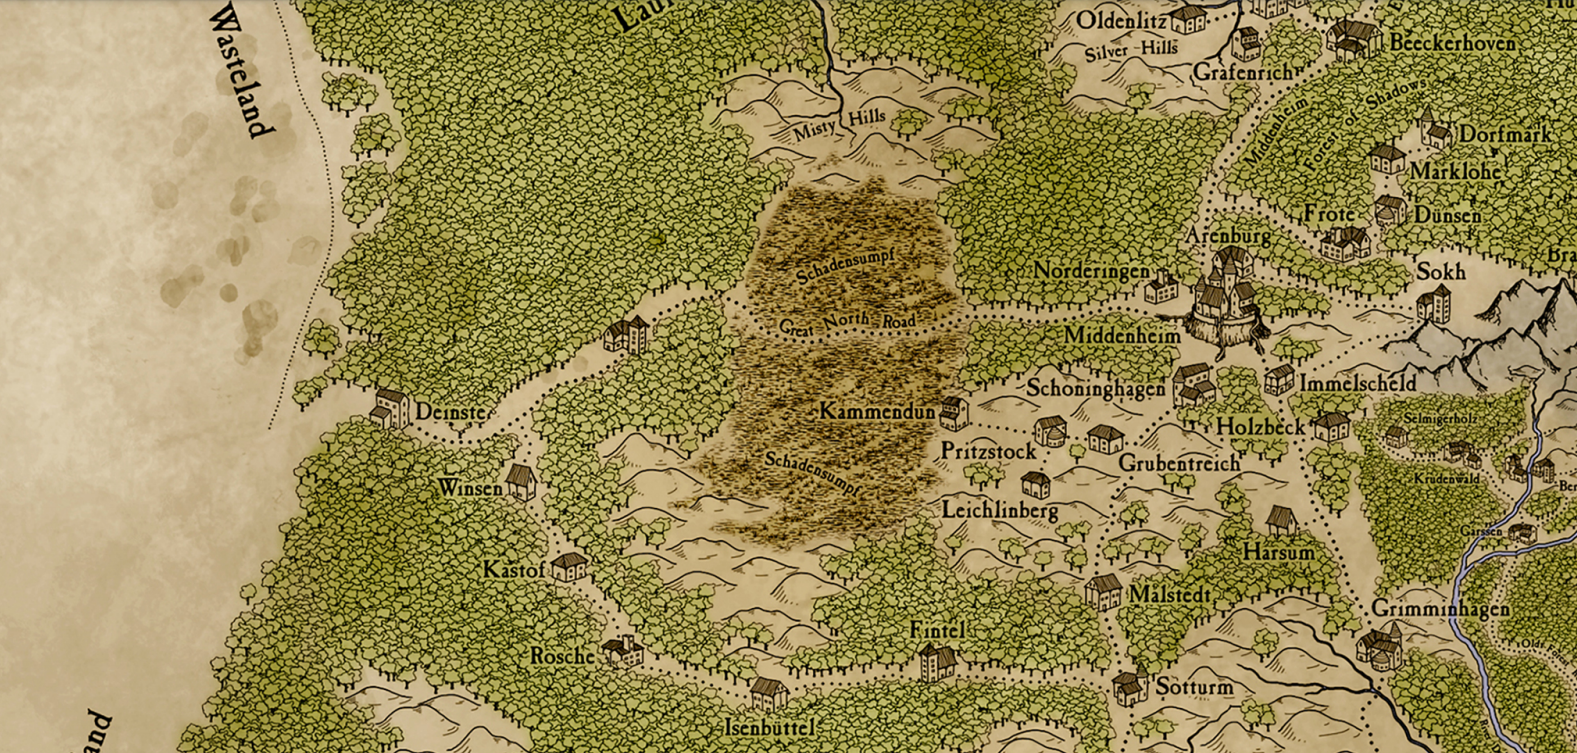
\includegraphics[width=\textwidth]{carte locale.png}
\section*{Noms de PNJs}
\subsection*{Impériaux}
\subsection*{Bretonniens}
\end{document}